% Final presentation: 15 main slides, results summary table, appendix (one slide per question).
% Build: pdflatex slides.tex (twice). Numbers: ../Reports/sources/data/values.tex (collect_values.py);
% plots: ../Reports/sources/figures/*.tex; field maps: figures/*.png (export_maps.sh).
\documentclass[aspectratio=169,10pt]{beamer}
\usetheme[progressbar=frametitle,numbering=fraction,block=fill]{metropolis}
\usepackage{booktabs,tabularx,amsmath,pgfplots,tikz}
\pgfplotsset{compat=1.18}
\definecolor{accent}{HTML}{254C58}\definecolor{warm}{HTML}{D1495B}
\setbeamercolor{frametitle}{bg=accent}\setbeamercolor{progress bar}{fg=warm}
\setbeamercolor{alerted text}{fg=warm}
% Generated by Reports/collect_values.py. Do not edit.
\newcommand{\AmpLin}{386}
\newcommand{\Ampflat}{343}
\newcommand{\Ampflatsev}{352}
\newcommand{\Ampflatsevsp}{374}
\newcommand{\Ampflatsp}{351}
\newcommand{\Amptrefoil}{345}
\newcommand{\Amptrefoilsp}{350}
\newcommand{\AnaC}{0.197031}
\newcommand{\AnaCbare}{0.1834}
\newcommand{\AnaCthick}{0.181271}
\newcommand{\AnaDeltaAl}{11.96}
\newcommand{\AnaDeltaCu}{9.35}
\newcommand{\AnaDrop}{7}
\newcommand{\AnaEb}{5.14}
\newcommand{\AnaEi}{4.894}
\newcommand{\AnaEirms}{3.46}
\newcommand{\AnaEithick}{4.502}
\newcommand{\AnaEorms}{1.71}
\newcommand{\AnaEvoid}{6.20}
\newcommand{\AnaEzero}{4.34}
\newcommand{\AnaIch}{1.179}
\newcommand{\AnaJc}{\ensuremath{4.89\cdot10^{-12}}}
\newcommand{\AnaJd}{0.0340}
\newcommand{\AnaLgap}{0.4043}
\newcommand{\AnaLtouch}{0.4019}
\newcommand{\AnaRatio}{\ensuremath{1.44\cdot10^{-10}}}
\newcommand{\AnaWd}{0.022}
\newcommand{\AnaWdShare}{0.09}
\newcommand{\Bmax}{15.6}
\newcommand{\Bsingle}{13.4}
\newcommand{\Cdefect}{0.197000}
\newcommand{\Cdefectfine}{0.196999}
\newcommand{\Cffive}{0.197032}
\newcommand{\Cfhund}{0.197032}
\newcommand{\Cfthou}{0.197032}
\newcommand{\Cgap}{0.197032}
\newcommand{\Cgapcoarse}{0.197044}
\newcommand{\Cgapfine}{0.197031}
\newcommand{\CondShare}{94}
\newcommand{\ConvRate}{0.22}
\newcommand{\Cqdefect}{0.196937}
\newcommand{\Cqdefectfine}{0.196935}
\newcommand{\Cqffive}{0.197032}
\newcommand{\Cqfhund}{0.197032}
\newcommand{\Cqfthou}{0.197032}
\newcommand{\Cqgap}{0.197032}
\newcommand{\Cqgapcoarse}{0.197044}
\newcommand{\Cqgapfine}{0.197031}
\newcommand{\Cqthick}{0.181272}
\newcommand{\Cqtouching}{0.197032}
\newcommand{\Cthick}{0.181272}
\newcommand{\Ctouching}{0.197032}
\newcommand{\Dofsdefect}{65\,900}
\newcommand{\Dofsdefectfine}{265\,156}
\newcommand{\Dofsffive}{64\,884}
\newcommand{\Dofsfhund}{64\,884}
\newcommand{\Dofsfthou}{64\,884}
\newcommand{\Dofsgap}{64\,884}
\newcommand{\Dofsgapcoarse}{16\,100}
\newcommand{\Dofsgapfine}{261\,058}
\newcommand{\Dofsthick}{76\,210}
\newcommand{\Dofstouching}{64\,880}
\newcommand{\EddyFE}{0.9}
\newcommand{\Edefect}{6.29}
\newcommand{\Edefectfine}{6.30}
\newcommand{\Effive}{4.873}
\newcommand{\Efhund}{4.873}
\newcommand{\Efthou}{4.873}
\newcommand{\Egap}{4.873}
\newcommand{\Egapcoarse}{4.846}
\newcommand{\Egapfine}{4.885}
\newcommand{\Ethick}{4.474}
\newcommand{\Etouching}{4.872}
\newcommand{\Hrad}{5.2}
\newcommand{\Ibalance}{\ensuremath{4\cdot10^{-14}}}
\newcommand{\IchFE}{1.179}
\newcommand{\IecAmp}{351}
\newcommand{\IecIs}{56.8}
\newcommand{\IecLam}{5.52}
\newcommand{\IecLamHot}{3.6}
\newcommand{\IecPc}{60.55}
\newcommand{\IecPcHot}{76.8}
\newcommand{\IecPs}{3.34}
\newcommand{\IecPsHot}{2.76}
\newcommand{\IecPt}{63.89}
\newcommand{\IecRac}{0.1739}
\newcommand{\IecRacHot}{0.2164}
\newcommand{\IecRcond}{0.16475}
\newcommand{\IecRcondHot}{0.2089}
\newcommand{\IecRs}{0.3448}
\newcommand{\IecTfour}{2.236}
\newcommand{\IecTheta}{89.2}
\newcommand{\IecThetaS}{77}
\newcommand{\IecTone}{0.476}
\newcommand{\IecTthree}{0.104}
\newcommand{\IecU}{46.5}
\newcommand{\IecUs}{19.9}
\newcommand{\IecX}{0.0568}
\newcommand{\IecYp}{0.15}
\newcommand{\IecYs}{0.31}
\newcommand{\IecYsp}{0.46}
\newcommand{\Ioneflat}{341}
\newcommand{\Ioneflatsev}{353}
\newcommand{\Ioneflatsevsp}{381}
\newcommand{\Ioneflatsp}{351}
\newcommand{\Ionetrefoil}{344}
\newcommand{\Ionetrefoilsp}{350}
\newcommand{\IratioFE}{\ensuremath{1.44\cdot10^{-10}}}
\newcommand{\IsPeak}{79}
\newcommand{\IsSum}{0.15}
\newcommand{\Isbase}{55.5}
\newcommand{\Isbox}{55.9}
\newcommand{\Iscoarse}{54.9}
\newcommand{\Isfdc}{0.0}
\newcommand{\Isffive}{5.7}
\newcommand{\Isfhund}{267.6}
\newcommand{\Isfine}{55.8}
\newcommand{\Isflat}{60.9}
\newcommand{\IsflatIone}{60.0}
\newcommand{\Isflatsev}{95.4}
\newcommand{\IsflatsevIone}{95.9}
\newcommand{\Isflatsevsp}{0.0}
\newcommand{\IsflatsevspIone}{0.0}
\newcommand{\Isflatsp}{0.0}
\newcommand{\IsflatspIone}{0.0}
\newcommand{\Islin}{55.5}
\newcommand{\Isliniso}{55.5}
\newcommand{\Isnl}{45.4}
\newcommand{\Isnlcoarse}{45.0}
\newcommand{\Isnldomforty}{45.4}
\newcommand{\Isnldomten}{45.4}
\newcommand{\Isnlfine}{45.5}
\newcommand{\Isnlhfive}{45.2}
\newcommand{\Isnlhtwenty}{45.5}
\newcommand{\Isnliso}{45.6}
\newcommand{\Issingle}{0.0}
\newcommand{\Isstranded}{55.6}
\newcommand{\Isstrandedfhund}{268.1}
\newcommand{\Istouching}{54.9}
\newcommand{\Istrefoil}{45.4}
\newcommand{\IstrefoilIone}{45.0}
\newcommand{\Istrefoilsp}{0.0}
\newcommand{\IstrefoilspIone}{0.0}
\newcommand{\Javg}{2.88}
\newcommand{\JcFE}{\ensuremath{4.87\cdot10^{-12}}}
\newcommand{\JdFE}{0.0339}
\newcommand{\Jmax}{3.07}
\newcommand{\Jscreen}{1.6}
\newcommand{\LamFE}{6.1}
\newcommand{\Lbase}{0.3943}
\newcommand{\Lbox}{0.3955}
\newcommand{\Lcoarse}{0.3922}
\newcommand{\Lfdc}{0.4010}
\newcommand{\Lffive}{0.4010}
\newcommand{\Lfhund}{0.2616}
\newcommand{\Lfine}{0.3952}
\newcommand{\Lflat}{0.4331}
\newcommand{\LflatIone}{0.4328}
\newcommand{\Lflatsev}{0.5722}
\newcommand{\LflatsevIone}{0.5724}
\newcommand{\Lflatsevsp}{0.6061}
\newcommand{\LflatsevspIone}{0.6061}
\newcommand{\Lflatsp}{0.4437}
\newcommand{\LflatspIone}{0.4437}
\newcommand{\Llin}{0.3943}
\newcommand{\Lliniso}{0.3943}
\newcommand{\Lnl}{0.3965}
\newcommand{\Lnlcoarse}{0.3944}
\newcommand{\Lnldomforty}{0.3965}
\newcommand{\Lnldomten}{0.3965}
\newcommand{\Lnlfine}{0.3975}
\newcommand{\Lnlhfive}{0.3966}
\newcommand{\Lnlhtwenty}{0.3965}
\newcommand{\Lnliso}{0.3965}
\newcommand{\Lsingle}{0.4003}
\newcommand{\Lstranded}{0.3947}
\newcommand{\Lstrandedfhund}{0.2670}
\newcommand{\Lterm}{0.3945}
\newcommand{\Ltouching}{0.3923}
\newcommand{\Ltrefoil}{0.3965}
\newcommand{\LtrefoilIone}{0.3965}
\newcommand{\Ltrefoilsp}{0.4006}
\newcommand{\LtrefoilspIone}{0.4006}
\newcommand{\MDofsbase}{295\,294}
\newcommand{\MDofsbox}{297\,138}
\newcommand{\MDofscoarse}{75\,856}
\newcommand{\MDofsfdc}{295\,294}
\newcommand{\MDofsffive}{295\,294}
\newcommand{\MDofsfhund}{295\,294}
\newcommand{\MDofsfine}{1\,169\,120}
\newcommand{\MDofsflat}{243\,780}
\newcommand{\MDofsflatIone}{243\,780}
\newcommand{\MDofsflatsev}{253\,538}
\newcommand{\MDofsflatsevIone}{253\,538}
\newcommand{\MDofsflatsevsp}{253\,538}
\newcommand{\MDofsflatsevspIone}{253\,538}
\newcommand{\MDofsflatsp}{243\,780}
\newcommand{\MDofsflatspIone}{243\,780}
\newcommand{\MDofslin}{295\,294}
\newcommand{\MDofsliniso}{295\,294}
\newcommand{\MDofsnl}{295\,294}
\newcommand{\MDofsnlcoarse}{75\,856}
\newcommand{\MDofsnldomforty}{295\,294}
\newcommand{\MDofsnldomten}{295\,294}
\newcommand{\MDofsnlfine}{1\,169\,120}
\newcommand{\MDofsnlhfive}{295\,294}
\newcommand{\MDofsnlhtwenty}{295\,294}
\newcommand{\MDofsnliso}{295\,294}
\newcommand{\MDofssingle}{295\,294}
\newcommand{\MDofsstranded}{295\,288}
\newcommand{\MDofsstrandedfhund}{295\,288}
\newcommand{\MDofstouching}{292\,266}
\newcommand{\MDofstrefoil}{295\,294}
\newcommand{\MDofstrefoilIone}{295\,294}
\newcommand{\MDofstrefoilsp}{295\,294}
\newcommand{\MDofstrefoilspIone}{295\,294}
\newcommand{\MeshBadGap}{0}
\newcommand{\MeshBadTouch}{24}
\newcommand{\MeshQminGap}{0.575}
\newcommand{\MeshQminTouch}{0.020}
\newcommand{\MeshTriGap}{297\,943}
\newcommand{\MeshTriTouch}{294\,915}
\newcommand{\MeshXlpeGap}{22\,228}
\newcommand{\MeshXlpeTouch}{22\,222}
\newcommand{\Nitflat}{10}
\newcommand{\NitflatIone}{10}
\newcommand{\Nitflatsev}{9}
\newcommand{\NitflatsevIone}{9}
\newcommand{\Nitflatsevsp}{10}
\newcommand{\NitflatsevspIone}{11}
\newcommand{\Nitflatsp}{10}
\newcommand{\NitflatspIone}{10}
\newcommand{\Nitlin}{1}
\newcommand{\Nitliniso}{1}
\newcommand{\Nitnl}{10}
\newcommand{\Nitnlcoarse}{10}
\newcommand{\Nitnldomforty}{10}
\newcommand{\Nitnldomten}{10}
\newcommand{\Nitnlfine}{10}
\newcommand{\Nitnlhfive}{10}
\newcommand{\Nitnlhtwenty}{10}
\newcommand{\Nitnliso}{10}
\newcommand{\Nittrefoil}{10}
\newcommand{\NittrefoilIone}{10}
\newcommand{\Nittrefoilsp}{10}
\newcommand{\NittrefoilspIone}{10}
\newcommand{\NktL}{0.382}
\newcommand{\PcPhase}{20.18}
\newcommand{\Pcbase}{60.55}
\newcommand{\Pcbox}{60.55}
\newcommand{\Pccoarse}{60.58}
\newcommand{\Pcfdc}{60.28}
\newcommand{\Pcffive}{60.28}
\newcommand{\Pcfhund}{75.76}
\newcommand{\Pcfine}{60.54}
\newcommand{\Pcflat}{77.44}
\newcommand{\PcflatIone}{72.36}
\newcommand{\Pcflatsev}{76.02}
\newcommand{\PcflatsevIone}{77.69}
\newcommand{\Pcflatsevsp}{73.63}
\newcommand{\PcflatsevspIone}{91.14}
\newcommand{\Pcflatsp}{76.37}
\newcommand{\PcflatspIone}{77.04}
\newcommand{\PcircFE}{3.16}
\newcommand{\Pclin}{60.55}
\newcommand{\Pcliniso}{60.55}
\newcommand{\Pcnl}{77.58}
\newcommand{\Pcnlcoarse}{77.38}
\newcommand{\Pcnldomforty}{77.59}
\newcommand{\Pcnldomten}{77.51}
\newcommand{\Pcnlfine}{77.65}
\newcommand{\Pcnlhfive}{77.92}
\newcommand{\Pcnlhtwenty}{77.40}
\newcommand{\Pcnliso}{77.21}
\newcommand{\Pcsingle}{60.55}
\newcommand{\Pcstranded}{60.26}
\newcommand{\Pcstrandedfhund}{60.26}
\newcommand{\Pctouching}{60.55}
\newcommand{\Pctrefoil}{77.58}
\newcommand{\PctrefoilIone}{74.07}
\newcommand{\Pctrefoilsp}{76.94}
\newcommand{\PctrefoilspIone}{76.94}
\newcommand{\PdInception}{16}
\newcommand{\PhaseSym}{0.0004}
\newcommand{\Psbase}{3.68}
\newcommand{\Psbox}{3.74}
\newcommand{\Pscoarse}{3.59}
\newcommand{\Psfdc}{0.00}
\newcommand{\Psffive}{0.04}
\newcommand{\Psfhund}{81.84}
\newcommand{\Psfine}{3.72}
\newcommand{\Psflat}{5.01}
\newcommand{\PsflatIone}{4.81}
\newcommand{\Psflatsev}{12.34}
\newcommand{\PsflatsevIone}{12.51}
\newcommand{\Psflatsevsp}{0.05}
\newcommand{\PsflatsevspIone}{0.05}
\newcommand{\Psflatsp}{0.41}
\newcommand{\PsflatspIone}{0.41}
\newcommand{\Pslin}{3.68}
\newcommand{\Psliniso}{3.68}
\newcommand{\Psnl}{3.03}
\newcommand{\Psnlcoarse}{2.96}
\newcommand{\Psnldomforty}{3.03}
\newcommand{\Psnldomten}{3.03}
\newcommand{\Psnlfine}{3.06}
\newcommand{\Psnlhfive}{3.02}
\newcommand{\Psnlhtwenty}{3.04}
\newcommand{\Psnliso}{3.04}
\newcommand{\Pssingle}{0.52}
\newcommand{\Psstranded}{3.70}
\newcommand{\Psstrandedfhund}{83.03}
\newcommand{\Pstouching}{3.62}
\newcommand{\Pstrefoil}{3.03}
\newcommand{\PstrefoilIone}{2.95}
\newcommand{\Pstrefoilsp}{0.43}
\newcommand{\PstrefoilspIone}{0.43}
\newcommand{\Ptbase}{64.23}
\newcommand{\Ptbox}{64.30}
\newcommand{\Ptcoarse}{64.17}
\newcommand{\Ptfdc}{60.28}
\newcommand{\Ptffive}{60.32}
\newcommand{\Ptfhund}{157.60}
\newcommand{\Ptfine}{64.27}
\newcommand{\Ptflat}{82.45}
\newcommand{\PtflatIone}{77.17}
\newcommand{\Ptflatsev}{88.36}
\newcommand{\PtflatsevIone}{90.20}
\newcommand{\Ptflatsevsp}{73.68}
\newcommand{\PtflatsevspIone}{91.20}
\newcommand{\Ptflatsp}{76.77}
\newcommand{\PtflatspIone}{77.45}
\newcommand{\Ptlin}{64.23}
\newcommand{\Ptliniso}{64.23}
\newcommand{\Ptnl}{80.61}
\newcommand{\Ptnlcoarse}{80.33}
\newcommand{\Ptnldomforty}{80.62}
\newcommand{\Ptnldomten}{80.55}
\newcommand{\Ptnlfine}{80.71}
\newcommand{\Ptnlhfive}{80.94}
\newcommand{\Ptnlhtwenty}{80.43}
\newcommand{\Ptnliso}{80.25}
\newcommand{\Ptsingle}{61.07}
\newcommand{\Ptstranded}{63.96}
\newcommand{\Ptstrandedfhund}{143.29}
\newcommand{\Pttouching}{64.17}
\newcommand{\Pttrefoil}{80.61}
\newcommand{\PttrefoilIone}{77.02}
\newcommand{\Pttrefoilsp}{77.36}
\newcommand{\PttrefoilspIone}{77.36}
\newcommand{\QsFrac}{94.6}
\newcommand{\Racbase}{0.1748}
\newcommand{\Racbox}{0.1750}
\newcommand{\Raccoarse}{0.1746}
\newcommand{\Racfdc}{0.1640}
\newcommand{\Racffive}{0.1641}
\newcommand{\Racfhund}{0.4288}
\newcommand{\Racfine}{0.1749}
\newcommand{\Racflat}{0.2244}
\newcommand{\RacflatIone}{0.2214}
\newcommand{\Racflatsev}{0.2404}
\newcommand{\RacflatsevIone}{0.2413}
\newcommand{\Racflatsevsp}{0.2005}
\newcommand{\RacflatsevspIone}{0.2097}
\newcommand{\Racflatsp}{0.2089}
\newcommand{\RacflatspIone}{0.2093}
\newcommand{\Raclin}{0.1748}
\newcommand{\Racliniso}{0.1748}
\newcommand{\Racnl}{0.2193}
\newcommand{\Racnlcoarse}{0.2186}
\newcommand{\Racnldomforty}{0.2194}
\newcommand{\Racnldomten}{0.2192}
\newcommand{\Racnlfine}{0.2196}
\newcommand{\Racnlhfive}{0.2202}
\newcommand{\Racnlhtwenty}{0.2189}
\newcommand{\Racnliso}{0.2184}
\newcommand{\Racsingle}{0.1662}
\newcommand{\Racstranded}{0.1740}
\newcommand{\Racstrandedfhund}{0.3899}
\newcommand{\Ractouching}{0.1746}
\newcommand{\Ractrefoil}{0.2193}
\newcommand{\RactrefoilIone}{0.2172}
\newcommand{\Ractrefoilsp}{0.2105}
\newcommand{\RactrefoilspIone}{0.2105}
\newcommand{\Rcbase}{0.1648}
\newcommand{\Rcbox}{0.1648}
\newcommand{\Rccoarse}{0.1648}
\newcommand{\Rcfdc}{0.1640}
\newcommand{\Rcffive}{0.1640}
\newcommand{\Rcfhund}{0.2061}
\newcommand{\Rcfine}{0.1647}
\newcommand{\Rcflat}{0.2107}
\newcommand{\RcflatIone}{0.2076}
\newcommand{\Rcflatsev}{0.2069}
\newcommand{\RcflatsevIone}{0.2078}
\newcommand{\Rcflatsevsp}{0.2004}
\newcommand{\RcflatsevspIone}{0.2096}
\newcommand{\Rcflatsp}{0.2078}
\newcommand{\RcflatspIone}{0.2082}
\newcommand{\Rclin}{0.1648}
\newcommand{\Rcliniso}{0.1648}
\newcommand{\Rcnl}{0.2111}
\newcommand{\Rcnlcoarse}{0.2105}
\newcommand{\Rcnldomforty}{0.2111}
\newcommand{\Rcnldomten}{0.2109}
\newcommand{\Rcnlfine}{0.2113}
\newcommand{\Rcnlhfive}{0.2120}
\newcommand{\Rcnlhtwenty}{0.2106}
\newcommand{\Rcnliso}{0.2101}
\newcommand{\Rcsingle}{0.1648}
\newcommand{\Rcstranded}{0.1640}
\newcommand{\Rcstrandedfhund}{0.1640}
\newcommand{\Rctouching}{0.1648}
\newcommand{\Rctrefoil}{0.2111}
\newcommand{\RctrefoilIone}{0.2089}
\newcommand{\Rctrefoilsp}{0.2094}
\newcommand{\RctrefoilspIone}{0.2094}
\newcommand{\RhoHot}{28}
\newcommand{\ScreenFE}{6.1}
\newcommand{\SkinFE}{0.45}
\newcommand{\TDofsnl}{149\,003}
\newcommand{\TcA}{92.52}
\newcommand{\TcB}{92.74}
\newcommand{\TcC}{92.74}
\newcommand{\Tcflat}{94.1}
\newcommand{\TcflatIone}{89.0}
\newcommand{\Tcflatsev}{88.7}
\newcommand{\TcflatsevIone}{90.3}
\newcommand{\Tcflatsevsp}{78.4}
\newcommand{\TcflatsevspIone}{93.5}
\newcommand{\Tcflatsp}{89.5}
\newcommand{\TcflatspIone}{90.1}
\newcommand{\Tclin}{76.7}
\newcommand{\Tcliniso}{75.8}
\newcommand{\Tcnl}{92.7}
\newcommand{\Tcnlcoarse}{91.7}
\newcommand{\Tcnldomforty}{92.8}
\newcommand{\Tcnldomten}{92.5}
\newcommand{\Tcnlfine}{93.1}
\newcommand{\Tcnlhfive}{94.2}
\newcommand{\Tcnlhtwenty}{92.0}
\newcommand{\Tcnliso}{91.2}
\newcommand{\Tctrefoil}{92.7}
\newcommand{\TctrefoilIone}{89.3}
\newcommand{\Tctrefoilsp}{90.0}
\newcommand{\TctrefoilspIone}{90.0}
\newcommand{\Tsflat}{17.42}
\newcommand{\TsflatIone}{17.27}
\newcommand{\Tsflatsev}{17.58}
\newcommand{\TsflatsevIone}{17.63}
\newcommand{\Tsflatsevsp}{17.15}
\newcommand{\TsflatsevspIone}{17.66}
\newcommand{\Tsflatsp}{17.25}
\newcommand{\TsflatspIone}{17.27}
\newcommand{\Tslin}{16.89}
\newcommand{\Tsliniso}{15.00}
\newcommand{\Tsnl}{17.37}
\newcommand{\Tsnlcoarse}{17.36}
\newcommand{\Tsnldomforty}{17.37}
\newcommand{\Tsnldomten}{17.35}
\newcommand{\Tsnlfine}{17.38}
\newcommand{\Tsnlhfive}{19.47}
\newcommand{\Tsnlhtwenty}{16.23}
\newcommand{\Tsnliso}{15.00}
\newcommand{\Tstrefoil}{17.37}
\newcommand{\TstrefoilIone}{17.26}
\newcommand{\Tstrefoilsp}{17.28}
\newcommand{\TstrefoilspIone}{17.28}
\newcommand{\Usingle}{19.5}
\newcommand{\Vmeandefect}{6.11}
\newcommand{\Vmeandefectfine}{6.14}
\newcommand{\VoidRatio}{1.42}
\newcommand{\Zrbase}{0.1748}
\newcommand{\dAmpSingle}{+5}
\newcommand{\dCana}{0.0007}
\newcommand{\dCbare}{\ensuremath{-6.9}}
\newcommand{\dCnkt}{\ensuremath{-10.4}}
\newcommand{\dCthick}{\ensuremath{-8.0}}
\newcommand{\dCtouch}{\ensuremath{9\cdot10^{-6}}}
\newcommand{\dEfine}{\ensuremath{-0.17}}
\newcommand{\dEgap}{\ensuremath{-0.43}}
\newcommand{\dEthick}{\ensuremath{-8.2}}
\newcommand{\dEtouch}{+0.014}
\newcommand{\dIs}{\ensuremath{-2.3}}
\newcommand{\dLNL}{+0.57}
\newcommand{\dLana}{\ensuremath{-1.0}}
\newcommand{\dLbox}{+0.31}
\newcommand{\dLfine}{+0.23}
\newcommand{\dLflat}{+53}
\newcommand{\dLfreq}{\ensuremath{-1.7}}
\newcommand{\dLfreqhund}{\ensuremath{-35}}
\newcommand{\dLnkt}{+2.7}
\newcommand{\dLstr}{+0.09}
\newcommand{\dLterm}{0.06}
\newcommand{\dLtouch}{+0.52}
\newcommand{\dNktMax}{+0.3}
\newcommand{\dNktMin}{\ensuremath{-3.4}}
\newcommand{\dNktflat}{\ensuremath{-2.1}}
\newcommand{\dNktflatsev}{\ensuremath{-3.4}}
\newcommand{\dNktflatsevsp}{\ensuremath{-1.6}}
\newcommand{\dNktflatsp}{+0.3}
\newcommand{\dNkttrefoil}{\ensuremath{-1.4}}
\newcommand{\dNkttrefoilsp}{\ensuremath{-0.0}}
\newcommand{\dPcNL}{+28.1}
\newcommand{\dPcirc}{\ensuremath{-5}}
\newcommand{\dPsNL}{\ensuremath{-17.7}}
\newcommand{\dPsfine}{+1.2}
\newcommand{\dPstouch}{+1.7}
\newcommand{\dPtNL}{+25.5}
\newcommand{\dPtSingle}{\ensuremath{-4.9}}
\newcommand{\dRacNL}{+25.5}
\newcommand{\dRacSingle}{\ensuremath{-4.9}}
\newcommand{\dRacbox}{+0.10}
\newcommand{\dRacfine}{+0.06}
\newcommand{\dRactouch}{+0.09}
\newcommand{\dRcstr}{\ensuremath{-0.48}}
\newcommand{\dRcstrhund}{\ensuremath{-20}}
\newcommand{\dTIone}{3.5}
\newcommand{\dTcAlow}{0.2}
\newcommand{\dTcBC}{0.00}
\newcommand{\dTcCoarse}{\ensuremath{-1.0}}
\newcommand{\dTcDom}{+0.07}
\newcommand{\dTcDomten}{\ensuremath{-0.27}}
\newcommand{\dTcFine}{+0.3}
\newcommand{\dTcIso}{1.6}
\newcommand{\dTcNL}{+16.0}
\newcommand{\dTcNkt}{+2.7}
\newcommand{\dTfiller}{2.1}
\newcommand{\dToneThick}{6.5}
\newcommand{\dTsemi}{0.8}
\newcommand{\dTsurf}{2.4}
\newcommand{\dTthick}{0.8}

\def\datadir{../Reports/sources/data}
\newcommand{\plot}[3]{{\def\figw{#1}\def\figh{#2}% Shared pgfplots style for the report and the slides. \figw / \figh set the size.
\providecommand{\figw}{0.95\linewidth}\providecommand{\figh}{5.2cm}
\providecommand{\datadir}{data}
\ifdefined\figwlen\else\newlength\figwlen\fi\setlength{\figwlen}{\figw}
\pgfplotsset{every axis/.append style={width=\figw,height=\figh,grid=major,
  grid style={gray!25},tick label style={font=\scriptsize},label style={font=\small},
  legend style={font=\scriptsize,draw=none,fill=white,fill opacity=0.85,text opacity=1}}}
\definecolor{cA}{HTML}{254C58}\definecolor{cB}{HTML}{D1495B}\definecolor{cC}{HTML}{EDAE49}
\input{../Reports/sources/figures/#3.tex}}}
\newcommand{\map}[2]{\includegraphics[width=#1,trim=150 0 150 0,clip]{figures/#2.png}}
\newcommand{\q}[1]{{\color{warm}\bfseries #1}}
\newcommand{\src}[1]{\par\vfill{\tiny\color{gray}#1}}
\newcolumntype{Y}{>{\raggedright\arraybackslash}X}
\title{Electromagnetic and thermal FE analysis of a 33 kV cable system}
\subtitle{NKT 1$\times$185/50 mm\textsuperscript{2} XLPE-AL, three single cores in trefoil, buried 1 m}
\author{Finite Elements for Electromagnetic Fields (H9x34A)}
\date{KU Leuven -- December 2026}

\begin{document}
\maketitle

% ============================================================ 1. cable and choices
\begin{frame}{Cable system and modelling choices \q{Q1.1--Q1.4}}
\begin{columns}[T]
\column{0.4\textwidth}\centering
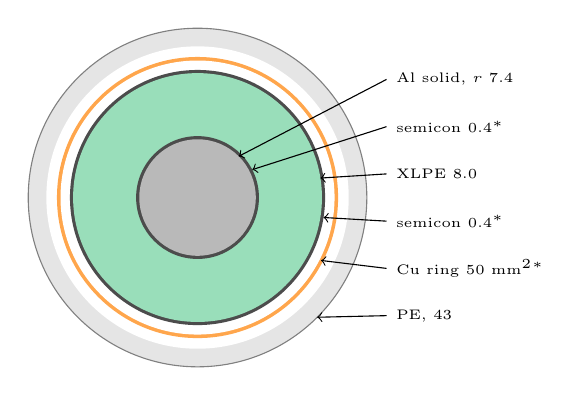
\begin{tikzpicture}[scale=0.1]
\fill[gray!20] (0,0) circle (21.5); \fill[white] (0,0) circle (19.2);
\fill[orange!70] (0,0) circle (17.85); \fill[white] (0,0) circle (17.4);
\fill[black!70] (0,0) circle (16.2); \fill[green!35!teal!40] (0,0) circle (15.8);
\fill[black!70] (0,0) circle (7.8); \fill[gray!55] (0,0) circle (7.4);
\draw[gray] (0,0) circle (21.5);
\foreach \r/\t/\y in {7.4/{Al solid, $r$ 7.4}/15, 7.8/semicon 0.4$^*$/9, 15.8/XLPE 8.0/3,
   16.2/semicon 0.4$^*$/-3, 17.6/{Cu ring 50 mm$^2$$^*$}/-9, 21.5/{PE, $\varnothing$43}/-15}
  \draw[->,thin] (24,\y) node[right,font=\tiny]{\t} -- ({\r*cos(\y*3)},{\r*sin(\y*3)});
\end{tikzpicture}\\
{\tiny radii in mm, to scale; $^*$ assumed}
\column{0.6\textwidth}\footnotesize
\begin{tabular}{@{}ll@{}}\toprule
Rating (NKT) & 33 kV, 350 A, 90\,$^\circ$C conductor\\
Laying (NKT) & trefoil touching, 1.0 m, 15\,$^\circ$C, 1.2 K\,m/W\\
Bonding & screens bonded at both ends (rating row)\\
Excitation & $\hat V=26.94$ kV, $\hat I=495$ A, ABC, 50 Hz (peak)\\\bottomrule
\end{tabular}\\[5pt]
\begin{itemize}\footnotesize
\item One parameterised geometry; \alert{all data are ONELAB parameters}
\item 0.5 mm soil gap between jackets: min.\ triangle quality \MeshQminTouch\ $\rightarrow$ \MeshQminGap
\item $\sigma_{\rm Al}$ fitted to $R_{DC}=0.164$ $\Omega$/km; polymers $\rho_T=3.5$ K\,m/W (IEC)
\item EM box $\pm$0.3 m inside a 40$\times$21 m soil domain: \alert{one mesh for all physics}
\end{itemize}
\end{columns}
\end{frame}

% ============================================================ 2. electric model
\begin{frame}{Electrodynamics: model and healthy stress \q{Q2.1, Q2.2, Q2.4}}
\begin{columns}[T]
\column{0.55\textwidth}\small
\[-\nabla\cdot\big((\sigma+j\omega\varepsilon)\nabla v\big)=0\ \text{ in the XLPE}\]
\begin{itemize}\small
\item Semicons ideal: $v=\hat V_k$ / $v=0$ on the XLPE interfaces (drop across them $\approx$\AnaDrop\ mV)
\item Grounded screens shield everything outside $\Rightarrow$ domain = 3 annuli
\item Each interface is one \emph{electrode}: unknown $U$, dual current $I$
\end{itemize}
\begin{tabular}{@{}lrr@{}}\toprule
$E_{\max}$ RMS [kV/mm] & cond.\ screen & core screen\\\midrule
Analytical & \AnaEirms & \AnaEorms\\
Limit (Eskom spec.) & 8 & 4\\\bottomrule
\end{tabular}\\[2pt]
Healthy insulation at $\le$43\% of the admissible stress.
\column{0.45\textwidth}\centering
\map{0.95\linewidth}{e_field}\\{\scriptsize $|\hat E|$ [V/m], peak \Egapfine\ kV/mm (analytical \AnaEi)}
\end{columns}
\end{frame}

% ============================================================ 3. electric verification
\begin{frame}{Electric verification: convergence, capacitance, conservation \q{Q2.3, Q2.6, Q2.7}}
\begin{columns}[T]
\column{0.56\textwidth}
\plot{\linewidth}{4.2cm}{convergence}\\
{\scriptsize Error concentrated at the conductor screen ($E\propto1/r$, constant per triangle) $\Rightarrow$ refine there.}
\column{0.44\textwidth}\small
\begin{tabular}{@{}lr@{}}\toprule
$C'$ [$\mu$F/km] & per phase\\\midrule
$2\pi\varepsilon/\ln(r_o/r_i)$ & \AnaC\\
FE energy / charge & \Cgap\\
NKT (max.) & 0.22\\\bottomrule
\end{tabular}\\[3pt]
Same $C$ from 5 to 5000 Hz.\\[3pt]
$|J_c/J_d|=\sigma/\omega\varepsilon=\AnaRatio$ in XLPE.\\
Electrode currents: $|I_{\rm in}+I_{\rm out}|/|I|=\Ibalance$; $|I|=\omega CV$ (\IchFE\ A/km).
\end{columns}
\end{frame}

% ============================================================ 4. defect and design
\begin{frame}{Air void and thicker insulation \q{Q2.5, Q2.8}}
\begin{columns}[T]
\column{0.34\textwidth}\centering
\map{\linewidth}{e_field_defect_zoom}\\{\scriptsize void $r$=0.25 mm at 8.8 mm, $\varepsilon_r$=1}
\column{0.66\textwidth}
\plot{\linewidth}{3.9cm}{radial_defect}\\[-3pt]\small
Void field \alert{\Vmeandefectfine--\Edefectfine\ kV/mm} ($\VoidRatio E_0$; cylinder theory $1.43E_0$) $>$
air breakdown \AnaEb--5.8 kV/mm $\Rightarrow$ \alert{partial discharges at rated voltage}: erosion, treeing, \alert{not withstood}.\\
\textbf{Design}: 9 mm XLPE (same $\varnothing$) $\Rightarrow$ $E_{\max}$ \Egap\ $\rightarrow$ \Ethick\ kV/mm ($-$8\%).
\end{columns}
\src{2D void = infinite channel (sphere: $1.25\times$): conservative. Breakdown: Paschen/Schumann, Kuffel et al.\ ch.~5.}
\end{frame}

% ============================================================ 5. magnetic model
\begin{frame}{Magnetoquasistatics: model, conductors, bonding \q{Q3.1--Q3.4}}
\small
\[\nabla\times(\nu\nabla\times\mathbf a)=\mathbf j,\qquad \mathbf j=-\sigma(j\omega\mathbf a+\mathbf u_r)\ \text{(massive)},\qquad \textstyle\int_{\Omega_m}j_z\,dA=I_m\]
\begin{columns}[T]
\column{0.5\textwidth}
\begin{itemize}\small
\item Screens do \emph{not} shield $\mathbf B$: whole EM box, $a_z=0$ at 0.3 m (balanced: $\propto1/r^2$; 0.6 m: $L$ \dLbox\%)
\item Solid Al $\Rightarrow$ \textbf{massive}: imposed $I_k$, eddy currents free ($\delta$=\AnaDeltaAl\ mm $>r$=7.4 mm)
\item Stranded ($J=I/A$): $R_{\rm cond}$ \dRcstr\% at 50 Hz, \dRcstrhund\% at 500 Hz
\end{itemize}
\column{0.5\textwidth}
\begin{itemize}\small
\item \textbf{Bonding} = one global $(U,I)$ per screen: both ends $U=0$; single point $I=0$
\item Only $\mathbf j=-j\omega\sigma\mathbf a$: net current set by the arbitrary $a$=0 reference at the box $\Rightarrow$ no defined circuit
\item Soil, semicons, fillers: $\sigma=0$ ($\delta\gg$ size)
\end{itemize}
\end{columns}
\end{frame}

% ============================================================ 6. magnetic results
\begin{frame}{Magnetic results vs IEC 60287 and datasheet \q{Q3.6--Q3.10}}
\begin{columns}[T]
\column{0.24\textwidth}\centering
\map{0.9\linewidth}{m_b}\\{\scriptsize $|\hat B|$, max \Bmax\ mT}\\[2pt]
\map{0.9\linewidth}{m_j}\\{\scriptsize $|\hat J|$ in Al and Cu}
\column{0.76\textwidth}\footnotesize
\begin{tabular}{@{}lrr@{}}\toprule
350 A, 50 Hz, 20\,$^\circ$C & FE & Reference\\\midrule
Losses conductors / screens [kW/km] & \Pcbase\ / \Psbase & \IecPc\ / \IecPs\ (IEC)\\
Screen current [A] & \Isbase & \IecIs\ (IEC)\\
$R_{DC}$ (FE at 0.01 Hz) [$\Omega$/km] & \Racfdc & 0.164 (NKT)\\
$R_{AC}=P/(3I^2)$ [$\Omega$/km] & \Racbase & \IecRac\ (IEC)\\
$L$ (touching) [mH/km] & \Ltouching & \NktL\ (NKT)\\\bottomrule
\end{tabular}\\[4pt]
$R_{AC}=R_{DC}(1+\SkinFE\%_{\,\rm skin+prox}+\ScreenFE\%_{\,\rm screens})$; IEC $y_s+y_p$ = \IecYsp\%.\\
$L=\int\nu|\hat b|^2/(3\hat I^2)$ = positive-sequence $L$; falls with $f$ (screen currents):
\Lfdc\ (DC), \Lbase\ (50 Hz), \Lfhund\ (500 Hz).
\end{columns}
\end{frame}

% ============================================================ 7. magnetic verification + design
\begin{frame}{Magnetic verification and loss reduction \q{Q3.5, Q3.11}}
\begin{columns}[T]
\column{0.52\textwidth}
\plot{\linewidth}{3.9cm}{mag_convergence}\\
{\scriptsize $h/\delta\le0.05$; mesh $\times$0.5: $R_{AC}$ \dRacfine\%, $L$ \dLfine\%, screen loss \dPsfine\% (thin ring: refine there)}
\column{0.48\textwidth}
\plot{0.95\linewidth}{4.0cm}{bonding}\\[-2pt]\small
Single-point bonding: losses \alert{\dPtSingle\%}; price: \Usingle\ V/km standing screen voltage.
\end{columns}
\end{frame}

% ============================================================ 8. thermal model
\begin{frame}{Coupled magneto-thermal model \q{Q4.1--Q4.3}}
\begin{columns}[T]
\column{0.5\textwidth}\small
\[-\nabla\cdot(\kappa\nabla T)=p=\tfrac12\sigma(T)|j\omega\hat{\mathbf a}+\hat{\mathbf u}_r|^2\]
\begin{itemize}\small
\item Heat source = time-averaged Joule loss, real: \texttt{<a>[...]}
\item Ground surface 1 m above: $-\kappa\partial_nT=h(T-15)$, $h$=10 W/(m$^2$K) (convection + radiation)
\item Sides $\pm$20 m: zero flux; bottom 20 m: $T$=15\,$^\circ$C ($T_{\max}$: $\approx$0.1 K vs 40 m)
\item Heat does not cancel like $\mathbf B$: line source, $\ln r$ decay $\Rightarrow$ domain $\gg$ EM box
\item One mesh: EM box nested in the soil, no interpolation; elements grow 15 cm/m
\end{itemize}
\column{0.5\textwidth}\centering
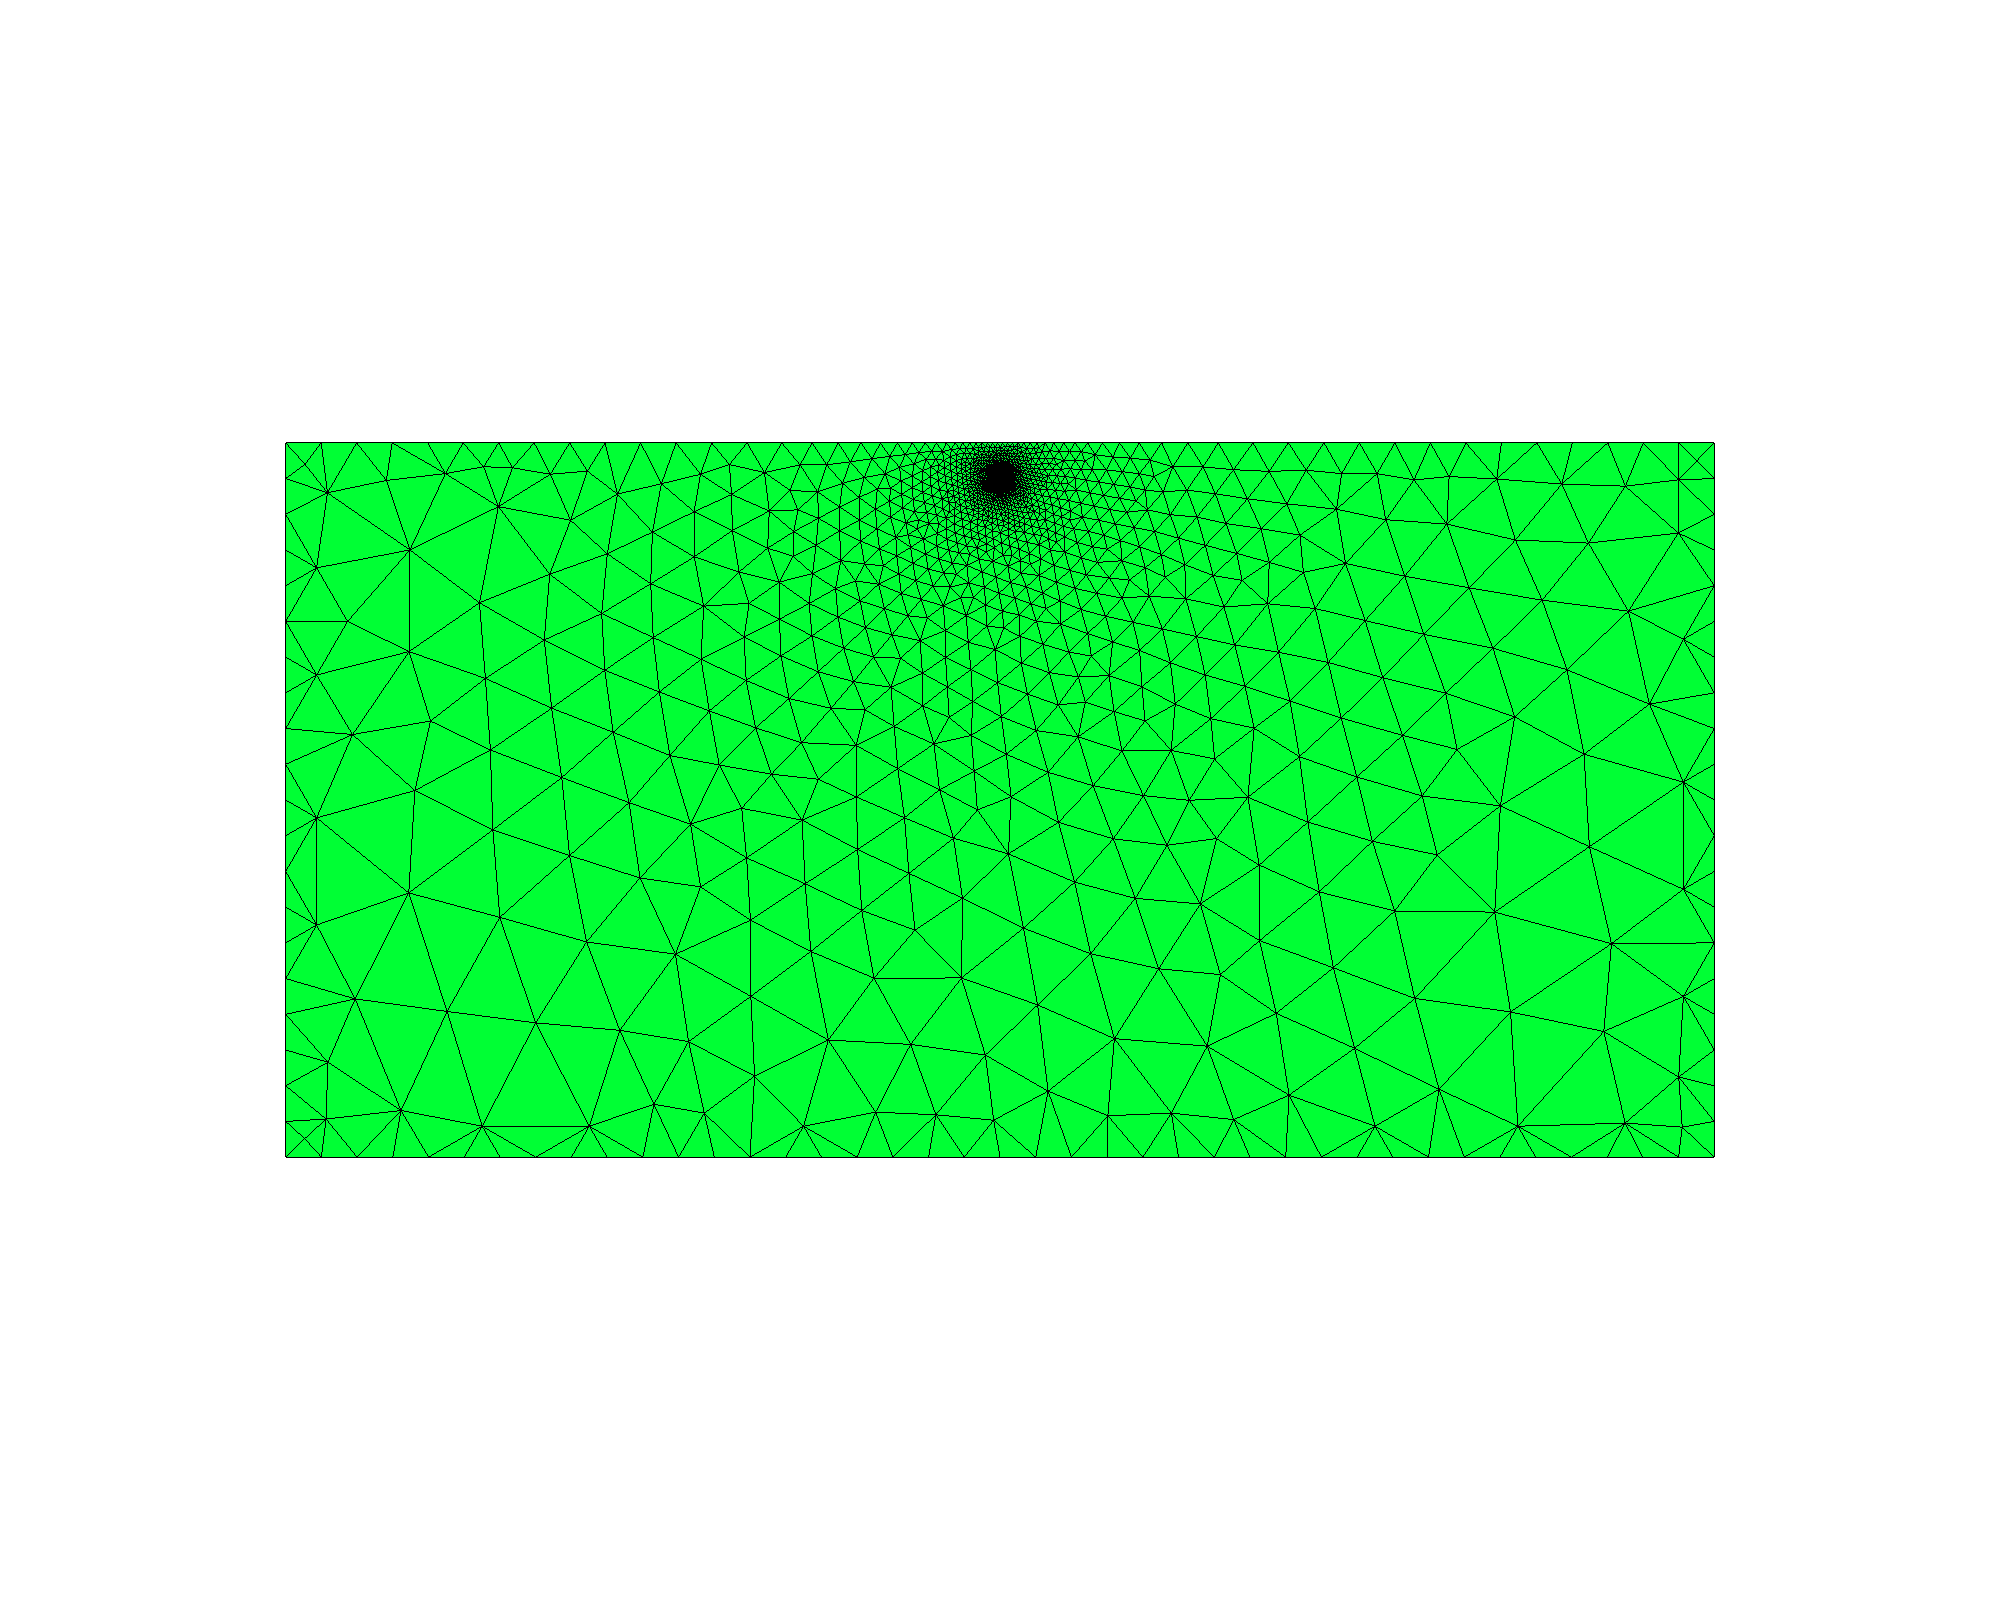
\includegraphics[width=\linewidth,trim=0 100 0 100,clip]{figures/mesh_domain.png}\\
{\scriptsize thermal mesh (40$\times$21 m); dense EM box at the cables}
\end{columns}
\end{frame}

% ============================================================ 9. temperatures
\begin{frame}{Temperatures at 350 A \q{Q4.4, Q4.5}}
\begin{columns}[T]
\column{0.26\textwidth}\centering
\map{0.8\linewidth}{t_cables_nl}\\{\scriptsize $T$ in the cables [$^\circ$C]}\\[2pt]
\map{0.8\linewidth}{t_soil_nl}\\{\scriptsize $T$ around them; ground surface on top}
\column{0.74\textwidth}\small
Hot spot \alert{\Tcnl\,$^\circ$C} in the lower cables B, C (A: $-$\dTcAlow\ K); XLPE limit 90\,$^\circ$C.
Max.\ ground-surface temperature \Tsnl\,$^\circ$C, above the trefoil.
Isothermal surface ($T$=15\,$^\circ$C): hot spot \Tcnliso\,$^\circ$C (convection adds \dTcIso\ K).\\[4pt]
\plot{0.9\linewidth}{4.3cm}{surface_profile}
\end{columns}
\end{frame}

% ============================================================ 10. validation
\begin{frame}{Validation: IEC 60287 and the NKT rating \q{Q4.6}}
\begin{columns}[T]
\column{0.47\textwidth}\small
\[\Delta\theta=W_c\left[T_1+(1+\lambda_1)(T_3+T_4)\right]\]
$T_1$=\IecTone, $T_3$=\IecTthree\ K\,m/W (polymers 3.5 K\,m/W),\\
$T_4=\frac{1.5}{\pi}\rho_T\left[\ln(2u)-0.630\right]$=\IecTfour\ K\,m/W (touching trefoil, $u=2L/D_e$)\\[3pt]
$R(\theta)$, $y_s$, $y_p$, $\lambda_1$ iterated with $\theta$; no dielectric loss.
\column{0.53\textwidth}\small
\begin{tabular}{@{}lrr@{}}\toprule
350 A & $\theta_c$ [$^\circ$C] & ampacity [A]\\\midrule
NKT datasheet & 90 & 350\\
IEC 60287 (isothermal surface) & \IecTheta & \IecAmp\\
FE $\sigma(T)$, isothermal surface & \Tcnliso & --\\
FE $\sigma(T)$, $h$=10 W/(m$^2$K) & \Tcnl & \Amptrefoil\\\bottomrule
\end{tabular}\\[4pt]
FE reproduces the rating within a few kelvin. Differences: convective surface (\dTcIso\ K),
2D conduction vs Kennelly + trefoil factor, FE screen losses, 0.5 mm gap.
\end{columns}
\end{frame}

% ============================================================ 11. nonlinear
\begin{frame}{Temperature-dependent conductivity \q{Q4.7--Q4.9}}
\begin{columns}[T]
\column{0.5\textwidth}
\plot{\linewidth}{4.3cm}{nl_history}\\
{\scriptsize $\|T_k-T_{k-1}\|_2/\|T_k\|_2<10^{-6}$ on all nodal temperatures: \Nitnl\ iterations, independent of the mesh}
\column{0.5\textwidth}\small
\begin{tabular}{@{}lrrr@{}}\toprule
& linear & $\sigma(T)$ & change\\\midrule
$P$ total [kW/km] & \Ptlin & \Ptnl & \dPtNL\%\\
$P$ screens [kW/km] & \Pslin & \Psnl & \dPsNL\%\\
$R_{AC}$ [$\Omega$/km] & \Raclin & \Racnl & \dRacNL\%\\
$L$ [mH/km] & \Llin & \Lnl & \dLNL\%\\
$T_{\max}$ [$^\circ$C] & \Tclin & \Tcnl & \dTcNL\ K\\\bottomrule
\end{tabular}\\[4pt]
Hotter Al $\Rightarrow$ lower $\sigma$ $\Rightarrow$ more loss. Screen loss \emph{drops} ($\lambda_1\approx X^2/R_s$).\\
\alert{Linear model is not conservative}: it would rate the cable at \AmpLin\ A instead of \Amptrefoil\ A.
\end{columns}
\end{frame}

% ============================================================ 12. section 5
\begin{frame}{Additional investigation: arrangement and bonding \q{Section 5}}
\begin{columns}[T]
\column{0.55\textwidth}
\plot{\linewidth}{4.6cm}{arrangement}
\column{0.45\textwidth}\scriptsize
\begin{tabular}{@{}lrrr@{}}\toprule
$\sigma(T)$, 350 A & $P_s$ [kW/km] & $L$ [mH/km] & $T_{\max}$\\\midrule
trefoil, both & \Pstrefoil & \Ltrefoil & \Tctrefoil\\
trefoil, single & \Pstrefoilsp & \Ltrefoilsp & \Tctrefoilsp\\
flat, both & \Psflat & \Lflat & \Tcflat\\
flat, single & \Psflatsp & \Lflatsp & \Tcflatsp\\
flat +70 mm, both & \Psflatsev & \Lflatsev & \Tcflatsev\\
flat +70 mm, single & \Psflatsevsp & \Lflatsevsp & \Tcflatsevsp\\\bottomrule
\end{tabular}\\[4pt]
\small Spacing cools, but with both ends bonded the screen losses quadruple and eat the gain;
single-point bonding removes them. All six FE ratings within \dNktMin\% \ldots\ \dNktMax\% of NKT.
\end{columns}
\src{Topic chosen by us (none assigned yet). Ampacity: two coupled runs per case, interpolated in $I^2$ to 90\,$^\circ$C.}
\end{frame}

% ============================================================ 13. design
\begin{frame}{Design proposals}
\footnotesize
\begin{tabular}{@{}p{38mm}p{52mm}p{44mm}@{}}\toprule
Proposal & Quantified gain & Price\\\midrule
9 mm XLPE (Q2.8) & $E_{\max}$ $-$8\%, more margin for voids & filler kept: $T_1$ +\dToneThick\% ($\approx$\dTthick\ K)\\
Single-point / cross-bonding (Q3.11) & losses \dPtSingle\%, ampacity \dAmpSingle\ A (trefoil) & standing voltage \Usingle\ V/km, SVLs\\
Flat, 70 mm apart, single point (S5) & ampacity \Ampflatsevsp\ A vs \Amptrefoil\ A & $\approx$3$\times$ wider trench, $L$ +53\%\\\bottomrule
\end{tabular}\\[8pt]
\textbf{Best arrangement:} for 350 A the rated trefoil is at its limit (FE \Tcnl\,$^\circ$C, within 3 K of 90\,$^\circ$C);
single-point bonding brings it to \Tctrefoilsp\,$^\circ$C. For more current, flat spaced with single-point or
cross-bonding gives the largest margin (\Ampflatsevsp\ A).
\end{frame}

% ============================================================ 14. conclusions
\begin{frame}{Conclusions}
\small
\begin{itemize}
\item \textbf{One geometry, two models} (electric; magneto-thermal), all inputs ONELAB parameters, \textbf{Run} reproduces every slide
\item \textbf{Verified}: $E_{\max}$ \dEfine\%, $C$ \dCana\% (analytical); $R_{\rm cond}$ vs IEC $y_s+y_p$; current balance \Ibalance; mesh, domain, frequency studies
\item \textbf{Validated}: $C$ $<$ NKT max; $R_{DC}$ 0.164; $L$ within NKT rounding; \textbf{350 A $\rightarrow$ \Tcnl\,$^\circ$C} vs NKT 90\,$^\circ$C and IEC \IecTheta\,$^\circ$C
\item Healthy insulation at 43\% of its limit; a 0.5 mm void discharges at rated voltage
\item $\sigma(T)$ adds \dPtNL\% losses and \dTcNL\ K: the linear model is unsafe for rating
\item Limits: 2D (no lay, no ends), constant soil properties (no drying), steady state
\end{itemize}
\end{frame}

% ============================================================ summary table
\begin{frame}{Results summary (Table 1)}
\scriptsize
\begin{tabularx}{\linewidth}{@{}lrrY@{}}\toprule
Quantity & FE (linear) & FE ($\sigma(T)$) & Reference$^*$\\\midrule
Max.\ field, conductor screen (kV/mm pk) & \Egapfine & -- & \AnaEi\ (analytical)\\
Max.\ field with defect (kV/mm pk, void) & \Edefectfine & -- & \AnaEvoid\ (analytical, $1.43E_0$)\\
Capacitance ($\mu$F/km) & 0.19703 & -- & 0.19703 (analytical); $\le$0.22 (NKT)\\
DC resistance ($\Omega$/km) & \Racfdc & -- & 0.164 (NKT max., 20\,$^\circ$C)\\
AC resistance ($\Omega$/km) & \Raclin & \Racnl & \IecRac\ at 20\,$^\circ$C; \IecRacHot\ at \IecTheta\,$^\circ$C (IEC)\\
Inductance (mH/km) & \Llin & \Lnl & \NktL\ (NKT, $X$=0.12 $\Omega$/km)\\
Losses (kW/km): cond.\ / sheaths / armour & \Pclin\ / \Pslin\ / -- & \Pcnl\ / \Psnl\ / -- & \IecPc\ / \IecPs\ at 20\,$^\circ$C; \IecPcHot\ / \IecPsHot\ hot (IEC)\\
Max.\ conductor temperature ($^\circ$C) & \Tclin & \Tcnl & 90 (NKT, at 350 A); \IecTheta\ (IEC)\\
Max.\ surface temperature ($^\circ$C) & \Tslin & \Tsnl & 15 (IEC: isothermal surface)\\
Nonlinear iterations & -- & \Nitnl & --\\\bottomrule
\end{tabularx}\\[5pt]
$^*$ analytical (Appendix B, IEC 60287) or datasheet (NKT), as stated. 350 A RMS, 50 Hz, 0.5 mm gap, massive Al,
both ends bonded, $h$=10 W/(m$^2$K), default mesh. Linear = $\sigma$ at 20\,$^\circ$C.
\end{frame}

% ================================================================= APPENDIX
\appendix
\begin{frame}[standout]Appendix: one slide per question\end{frame}

\begin{frame}{Q1.1 Construction and material properties}
\tiny
\begin{tabular}{@{}lrl@{\hskip 10pt}lrrrl@{}}\toprule
Region & $r_o$ [mm] & basis & Material & $\varepsilon_r$ & $\sigma$ [S/m] & $\kappa$ [W/mK] & source\\\midrule
Al conductor & 7.40 & NKT & Al & -- & $3.544\cdot10^7$, $\alpha$ 0.0039 & 237 & fitted; Lee; course\\
Inner semicon & 7.80 & assumed & Cu & -- & $5.80\cdot10^7$, $\alpha$ 0.00386 & 402 & IEC; course\\
XLPE & 15.80 & NKT 8 mm & semicon & 2.25 & $2\cdot10^{-3}$ & 0.286 & Lee, OES; IEC\\
Outer semicon & 16.20 & assumed & XLPE & 2.5 & $10^{-18}$ & 0.286 & IEC; course\\
Inner filler & 17.40 & assumed & PE, fillers & 2.25 & $10^{-18}$ / 0 & 0.286 & IEC; assumption\\
Cu ring 50 mm$^2$ & 17.85 & area kept & soil & 10 & $10^{-2}$ & 0.833 & course; NKT 1.2 K\,m/W\\
Outer filler & 19.20 & NKT $\varnothing$38.4 & air (void) & 1 & $10^{-15}$ & -- & assumption\\
PE sheath & 21.50 & NKT $\varnothing$43 & & & & & \\\bottomrule
\end{tabular}\\[6pt]
\small Rating: 350 A, 90\,$^\circ$C, direct burial 1.0 m, 15\,$^\circ$C, 1.2 K\,m/W, trefoil touching, both ends bonded. All $\mu_r=1$.
\end{frame}

\begin{frame}{Q1.2 Environment}
\small
\begin{itemize}
\item Homogeneous soil per the NKT rating: 15\,$^\circ$C, $\kappa=0.833$ W/(m\,K), trefoil centre 1.0 m deep
\item EM: $\varepsilon_r$=10, $\sigma$=0.01 S/m (course App.~C) -- shielded (electric), $\delta$=712 m (magnetic)
\item Air above the ground surface: 15\,$^\circ$C, $h$=10 W/(m$^2$K); no soil drying (constant $\kappa$)
\end{itemize}
\centering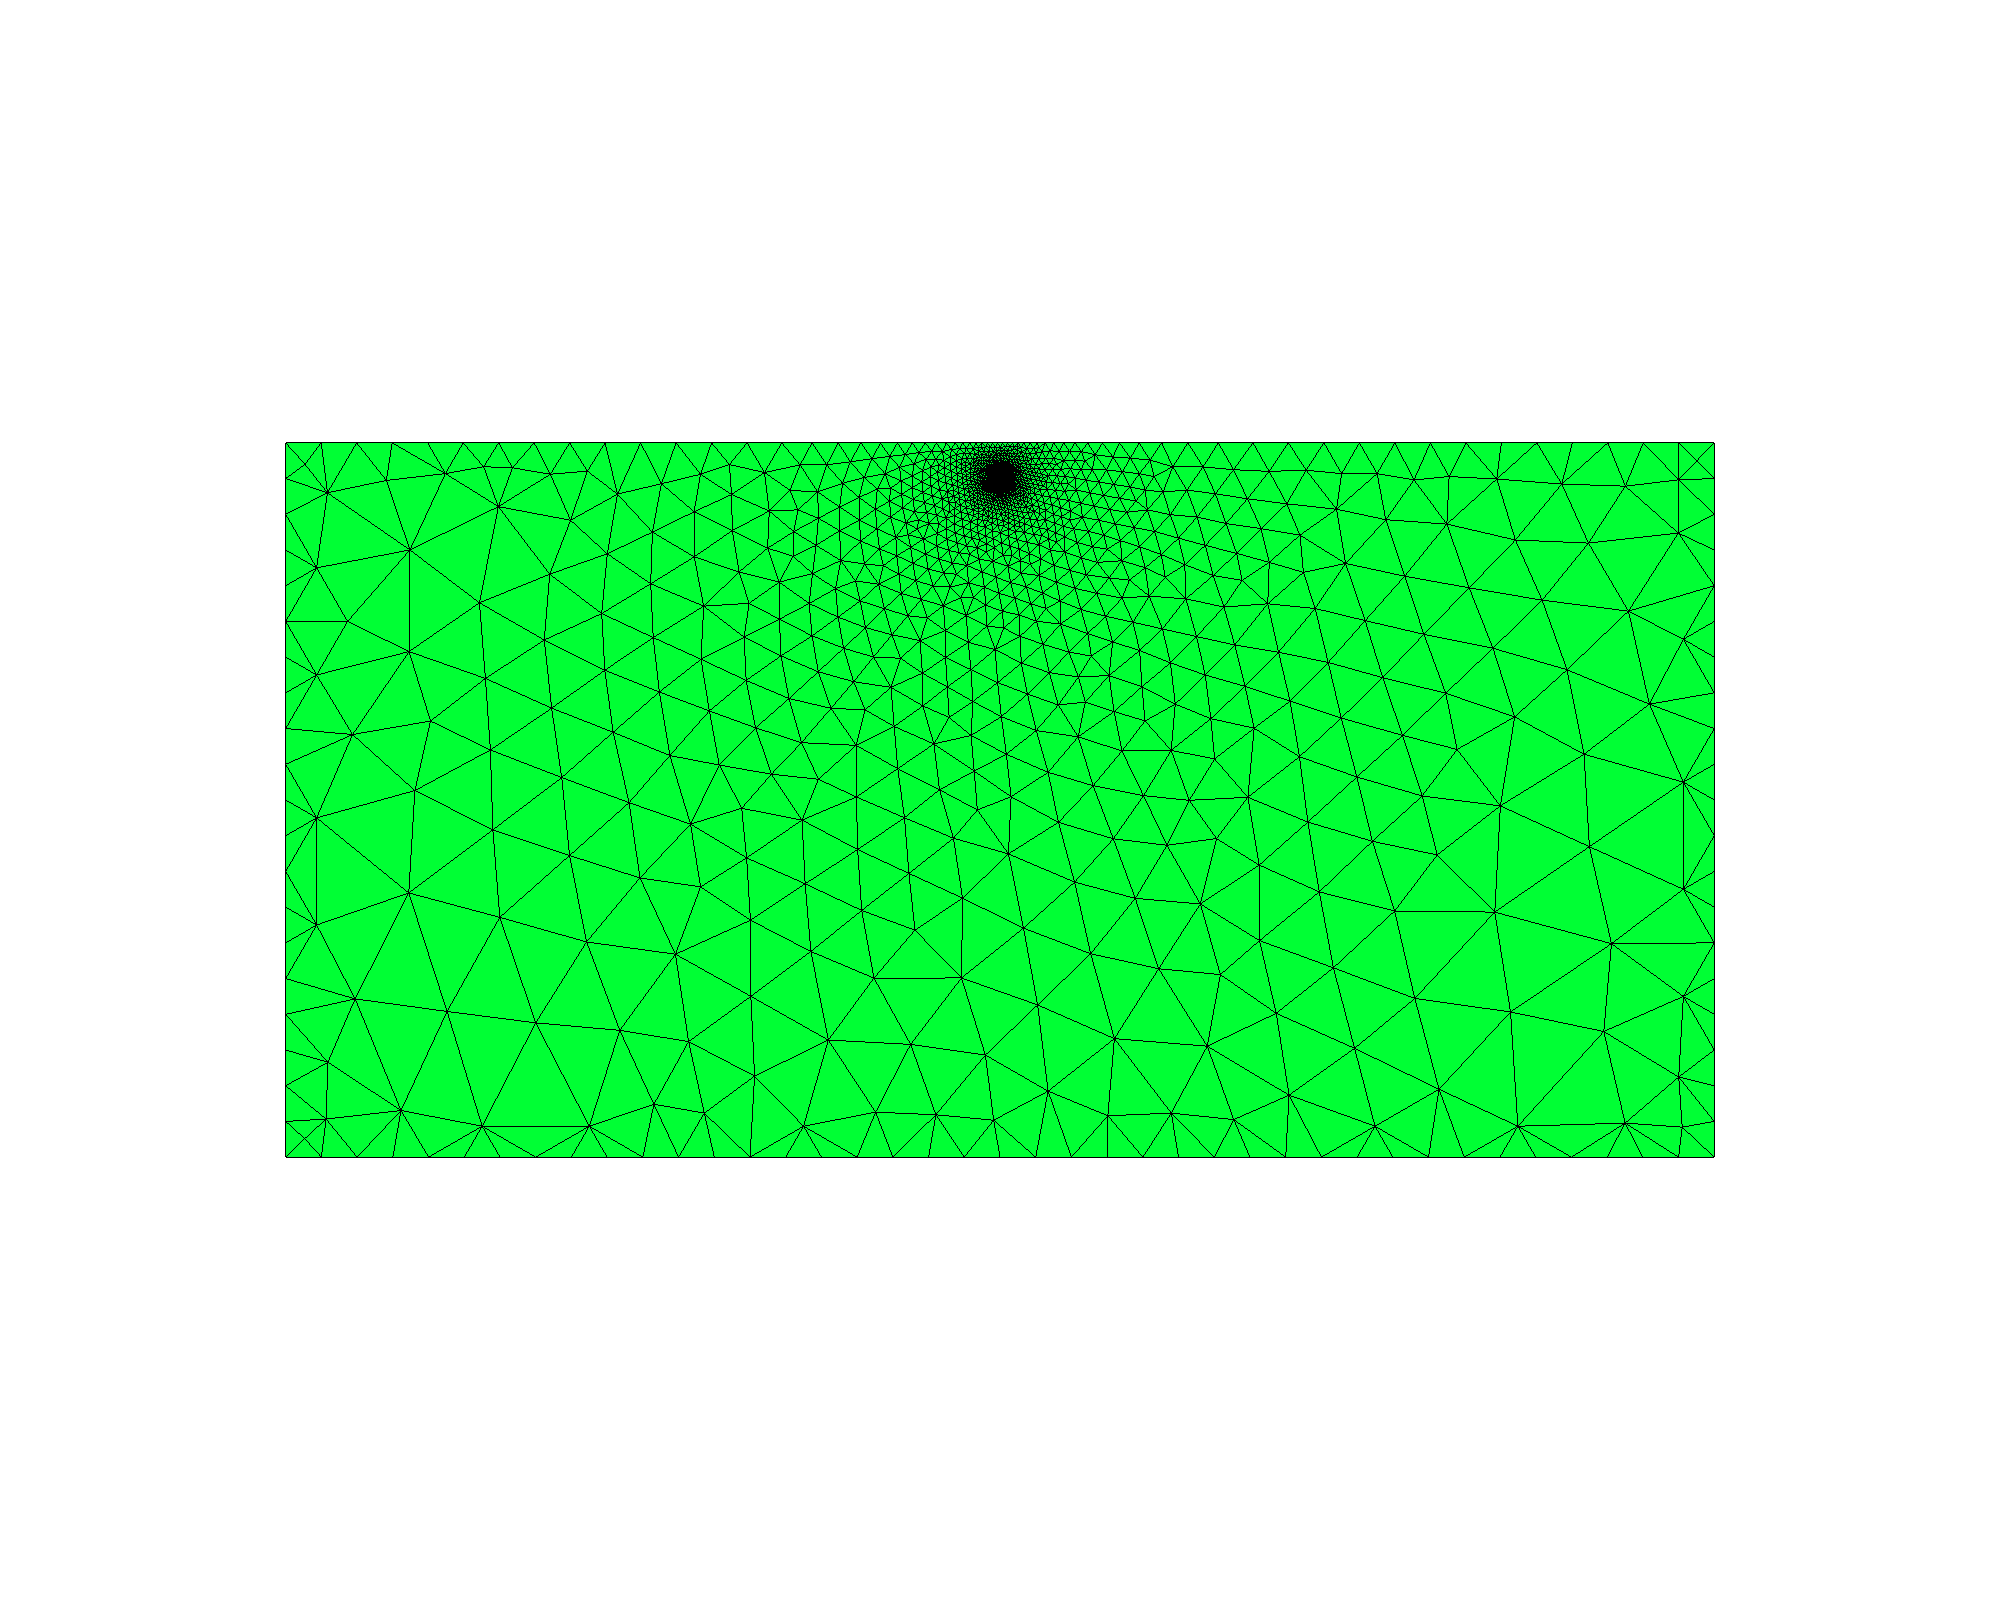
\includegraphics[width=0.45\linewidth,trim=0 100 0 100,clip]{figures/mesh_domain.png}
\end{frame}

\begin{frame}{Q1.3 Sheath bonding}
\small
\begin{itemize}
\item \textbf{Both ends bonded}, ideal earth leads (NKT rating row): circulating current allowed
\item Implemented as $U=0$ per copper screen $\Rightarrow I_s$ = \Isbase\ A RMS at 20\,$^\circ$C
\item Alternative: single point ($I=0$), Q3.11 and Section 5. No armour, no pipe.
\end{itemize}
\end{frame}

\begin{frame}{Q1.4 Excitation}
\small
\[\hat V_k=\tfrac{\sqrt2\,33}{\sqrt3}e^{-j2\pi k/3}=26.944\,e^{-j2\pi k/3}\ \mathrm{kV},\qquad
\hat I_k=\sqrt2\,350\,e^{-j2\pi k/3}=494.97\,e^{-j2\pi k/3}\ \mathrm{A}\]
A, B, C = 0, $-120^\circ$, $+120^\circ$; 50 Hz; $x(t)=\Re\{\hat xe^{j\omega t}\}$.
Voltages drive the electric model, currents the magnetic one. Reported: RMS values, time-averaged losses.
\end{frame}

\begin{frame}{Q2.1 Domain, equations, boundary conditions}
\begin{columns}[T]\column{0.55\textwidth}\small
\begin{itemize}
\item $-\nabla\cdot((\sigma+j\omega\varepsilon)\nabla v)=0$ in XLPE (41--43) + void (44)
\item Electrodes: $U=\hat V_k$ on 101--103, $U=0$ on 111--113
\item Truncation at the grounded core screen: outside regions cannot influence the insulation field
\item Weak form: \texttt{Galerkin} $\sigma$ + \texttt{DtDof} $\varepsilon$ + \texttt{GlobalTerm} $[-I,U]$
\end{itemize}
\column{0.45\textwidth}\centering\map{\linewidth}{e_potential}\\{\scriptsize $\Re(v)$ [V]}
\end{columns}
\end{frame}

\begin{frame}{Q2.2 Geometric simplifications}
\small
\begin{tabular}{@{}lr@{}}\toprule
Simplification & Effect\\\midrule
0.5 mm gap vs touching & $E_{\max}$ \dEtouch\%, $C$ $<$\dCtouch\%\\
Ideal semicons & drop $\approx$\AnaDrop\ mV ($3\cdot10^{-7}V$)\\
Voltage at 7.4 mm instead of 7.8 mm & $C$ \dCbare\% (screen thickness matters)\\
Metals, fillers, PE, soil not solved & exactly zero (shielded)\\\bottomrule
\end{tabular}
\end{frame}

\begin{frame}{Q2.3 Mesh convergence}
\begin{columns}[T]\column{0.6\textwidth}\plot{\linewidth}{4.4cm}{convergence}
\column{0.4\textwidth}\scriptsize
\begin{tabular}{@{}rrr@{}}\toprule
DoFs & $E_{\max}$ & $C'$\\\midrule
\Dofsgapcoarse & \Egapcoarse & \Cgapcoarse\\
\Dofsgap & \Egap & \Cgap\\
\Dofsgapfine & \Egapfine & \Cgapfine\\\bottomrule
\end{tabular}\\[4pt]\small $C$ converged; $E_{\max}$ needs local refinement at the conductor screen (and around a void).
\end{columns}
\end{frame}

\begin{frame}{Q2.4 Admissible field}
\small No NKT value: 8 kV/mm RMS (conductor screen) and 4 kV/mm RMS (core screen), Eskom 240-56030625.
Healthy: \AnaEirms\ / \AnaEorms\ kV/mm RMS $\Rightarrow$ within limits.\\[4pt]
\centering\map{0.38\linewidth}{e_field}
\end{frame}

\begin{frame}{Q2.5 Defect: maps with and without void}
\begin{columns}[T]
\column{0.25\textwidth}\centering\map{\linewidth}{e_field}\\{\scriptsize $|E|$ healthy}
\column{0.25\textwidth}\centering\map{\linewidth}{e_field_defect_zoom}\\{\scriptsize $|E|$ with void}
\column{0.25\textwidth}\centering\map{\linewidth}{e_jdisp}\\{\scriptsize $|J_d|$ healthy}
\column{0.25\textwidth}\centering\map{\linewidth}{e_jdisp_defect_zoom}\\{\scriptsize $|J_d|$ with void}
\end{columns}
\small Air void 0.5 mm, 0.75 mm from the conductor screen; $E_{\rm void}$ \Vmeandefectfine\ (mean) / \Edefectfine\ (max) kV/mm
$>$ $E_b$ \AnaEb--5.8 kV/mm $\Rightarrow$ PD inception $\approx$\PdInception\ kV $<U_0$=19 kV.
\end{frame}

\begin{frame}{Q2.6 Current densities and conservation}
\begin{columns}[T]\column{0.35\textwidth}\centering\map{\linewidth}{e_jdisp}
\column{0.65\textwidth}\small
XLPE: $|J_d|$=\AnaJd, $|J_c|$=\AnaJc\ A/m$^2$ peak: displacement dominates
(insulators, air); conduction dominates in semicons ($3\cdot10^5\times$), metals, soil.\\[4pt]
Per phase $|I_{\rm in}+I_{\rm out}|/|I_{\rm in}|\le\Ibalance$: exact global balance (sum of test functions = 1);
normal $J$ jumps between linear elements locally.
\end{columns}
\end{frame}

\begin{frame}{Q2.7 Capacitance}
\small $C'=2\pi\varepsilon_0\varepsilon_r/\ln(r_o/r_i)$, $r_i$=7.8, $r_o$=15.8 mm (XLPE interfaces; semicons are the electrodes) = \AnaC\ $\mu$F/km.\\[4pt]
FE energy \Cgap, charge \Cqgap; NKT $\le$0.22. 5/50/500/5000 Hz: \Cffive, \Cgap, \Cfhund, \Cfthou\ $\Rightarrow$
frequency independent: $(\sigma+j\omega\varepsilon)$ uniform per region cancels (no dispersion modelled).
\end{frame}

\begin{frame}{Q2.8 Electric design}
\begin{columns}[T]\column{0.6\textwidth}\plot{\linewidth}{4.4cm}{radial_thick}
\column{0.4\textwidth}\small 9 mm XLPE, same outer diameter: $E_{\max}$ \Egap\ $\rightarrow$ \Ethick\ kV/mm, $C$ $-$8\%.
Same $T_1$ here (filler and XLPE same $\kappa$); with the filler kept: $T_1$ +\dToneThick\%.
\end{columns}
\end{frame}

\begin{frame}{Q3.1 Domain, equations, boundary conditions, sources}
\small
\begin{itemize}
\item $\nabla\times\nu\nabla\times\mathbf a=\mathbf j$ in the $0.6\times0.6$ m EM box; $a_z=0$ on its edge
\item Massive Al, Cu: $\mathbf j=-\sigma(j\omega\mathbf a+\mathbf u_r)$, one $\mathbf u_r$ per region; rest $\sigma=0$, $\mu_r=1$
\item Phase currents: \texttt{Current\_2D} on the global $I$ of each Al region
\item Box edge: $|B|<1\%$ of peak; 0.6 m box changes $L$ by \dLbox\%
\end{itemize}
\end{frame}

\begin{frame}{Q3.2 Stranded vs massive}
\small $\delta_{\rm Al}$=\AnaDeltaAl\ mm $>$ $r$=7.4 mm.\\[4pt]
\begin{tabular}{@{}lrrr@{}}\toprule
& $R_{\rm cond}$ [$\Omega$/km] & $P_{\rm screen}$ [kW/km] & $L$ [mH/km]\\\midrule
Stranded 50 Hz & \Rcstranded & \Psstranded & \Lstranded\\
Massive 50 Hz & \Rcbase & \Psbase & \Lbase\\
Stranded 500 Hz & \Rcstrandedfhund & \Psstrandedfhund & \Lstrandedfhund\\
Massive 500 Hz & \Rcfhund & \Psfhund & \Lfhund\\\bottomrule
\end{tabular}\\[4pt]
Solid Al (NKT) $\Rightarrow$ massive; small difference at 50 Hz, large at 500 Hz.
\end{frame}

\begin{frame}{Q3.3 Bonding with global quantities}
\small
\begin{itemize}
\item Both ends: \texttt{Voltage\_2D} $U$=0 $\Rightarrow$ $I_s$ = \Isbase\ A RMS (IEC \IecIs\ A)
\item Single point: \texttt{Current\_2D} $I$=0 $\Rightarrow$ standing voltage \Usingle\ V/km (IEC $XI$=\IecUs)
\item $\mathbf j=-j\omega\sigma\mathbf a$ only: implicitly $U=0$ relative to the arbitrary box reference; net current depends on the truncation; $I=0$ impossible
\item Check: $|\sum I_{\rm screens}|=\IsSum$ A of \IsPeak\ A: nothing returns through the box edge
\end{itemize}
\end{frame}

\begin{frame}{Q3.4 Simplifications}
\small
\begin{itemize}
\item Gap vs touching: $L$ \dLtouch\%, $R_{AC}$ \dRactouch\%, screen loss \dPstouch\%
\item Wires + tape $\to$ equal-area ring: DC resistance kept, lay ignored
\item Semicons, fillers, soil $\sigma$=0: negligible ($\delta\gg$ size)
\item Section 2's ``XLPE only'' is \textbf{not} valid: $\mathbf B$ is not shielded
\end{itemize}
\end{frame}

\begin{frame}{Q3.5 Mesh and convergence}
\begin{columns}[T]\column{0.55\textwidth}\plot{\linewidth}{4.3cm}{mag_convergence}
\column{0.45\textwidth}\scriptsize
\begin{tabular}{@{}rrrr@{}}\toprule
DoFs & $R_{AC}$ & $L$ & $P_s$\\\midrule
\MDofscoarse & \Raccoarse & \Lcoarse & \Pscoarse\\
\MDofsbase & \Racbase & \Lbase & \Psbase\\
\MDofsfine & \Racfine & \Lfine & \Psfine\\\bottomrule
\end{tabular}\\[4pt]\small $h/\delta\le0.05$; refine inside the 0.45 mm screen.
\end{columns}
\end{frame}

\begin{frame}{Q3.6 Magnetic flux density}
\centering\map{0.45\linewidth}{m_b}\\\small Peak \Bmax\ mT on the conductor surfaces facing the trefoil centre.
\end{frame}

\begin{frame}{Q3.7 Current density}
\begin{columns}[T]
\column{0.5\textwidth}\centering\map{0.8\linewidth}{m_j}\\{\scriptsize both ends bonded}
\column{0.5\textwidth}\centering\map{0.8\linewidth}{m_j_single}\\{\scriptsize single point: eddies only}
\end{columns}
\end{frame}

\begin{frame}{Q3.8 Joule losses per part}
\small
\begin{tabular}{@{}lrrr@{}}\toprule
{[kW/km], 20\,$^\circ$C} & both ends & single point & IEC\\\midrule
Al conductors & \Pcbase & \Pcsingle & \IecPc\\
Cu screens & \Psbase & \Pssingle & \IecPs\\
Armour / pipe / soil & -- / -- / 0 & -- & --\\
Total & \Ptbase & \Ptsingle & \IecPt\\\bottomrule
\end{tabular}\\[4pt]
$p=|\hat j|^2/(2\sigma)$ with the total current density. At operating temperature: Q4.8.
\end{frame}

\begin{frame}{Q3.9 AC resistance}
\small $R_{AC}=P_{\rm tot}/(3I^2)$ = \Racbase\ $\Omega$/km; conductors only \Rcbase; DC \Racfdc\ (NKT 0.164).\\[4pt]
Skin + proximity +\SkinFE\% (IEC \IecYsp\%); screens +\ScreenFE\% (IEC $\lambda_1'$ \IecLam\% + eddy).
At operating temperature: \Racnl\ $\Omega$/km (Q4.8).
\end{frame}

\begin{frame}{Q3.10 Inductance}
\small $L=\int\nu|\hat b|^2/(3\hat I^2)$ = positive-sequence inductance (balanced, symmetric).\\[4pt]
\begin{tabular}{@{}lrrrr@{}}\toprule
$f$ [Hz] & 0.01 & 5 & 50 & 500\\\midrule
$L$ [mH/km] & \Lfdc & \Lffive & \Lbase & \Lfhund\\\bottomrule
\end{tabular}\\[4pt]
Decreases with $f$ (screen + eddy currents). NKT \NktL\ (0.366--0.398) vs FE touching \Ltouching.
\end{frame}

\begin{frame}{Q3.11 Loss-reducing design}
\begin{columns}[T]\column{0.5\textwidth}\centering\plot{0.95\linewidth}{4.4cm}{bonding}
\column{0.5\textwidth}\small Single-point (or cross-) bonding: losses \dPtSingle\%, $R_{AC}$ \Racbase\ $\rightarrow$ \Racsingle.
Trade-off: \Usingle\ V/km standing voltage. Thermal gain: \dAmpSingle\ A (Section 5).
\end{columns}
\end{frame}

\begin{frame}{Q4.1 Equations and heat source}
\small
\[-\nabla\cdot(\kappa\nabla T)=p,\qquad p=\frac{|\hat{\mathbf j}|^2}{2\sigma}=\tfrac12\sigma(T)\,|j\omega\hat{\mathbf a}+\hat{\mathbf u}_r|^2\ \text{(time average, peak phasors)}\]
\begin{itemize}
\item \texttt{<a>[\,0.5*sigma[]*SquNorm[Dt[\{a\}]+\{ur\}]\,]}: evaluated in the complex magnetic system, returns a real number
\item Steady state; dielectric loss $\omega CU_0^2\tan\delta=\AnaWd$ W/m per phase (\AnaWdShare\%): neglected (IEC)
\end{itemize}
\end{frame}

\begin{frame}{Q4.2 Thermal domain and boundary conditions}
\begin{columns}[T]\column{0.5\textwidth}\small
\begin{itemize}
\item Cooling: conduction through the soil to the ground surface, then convection + radiation to air
\item Surface: $h$=10 W/(m$^2$K) (natural convection 2--5 + radiation $4\varepsilon\sigma_{SB}T^3\approx5$)
\item Sides $\pm$20 m adiabatic; bottom 20 m: $T$=15\,$^\circ$C
\item \QsFrac\% of the heat leaves through the surface
\item One mesh (nested EM box, no interpolation)
\end{itemize}
\column{0.5\textwidth}\centering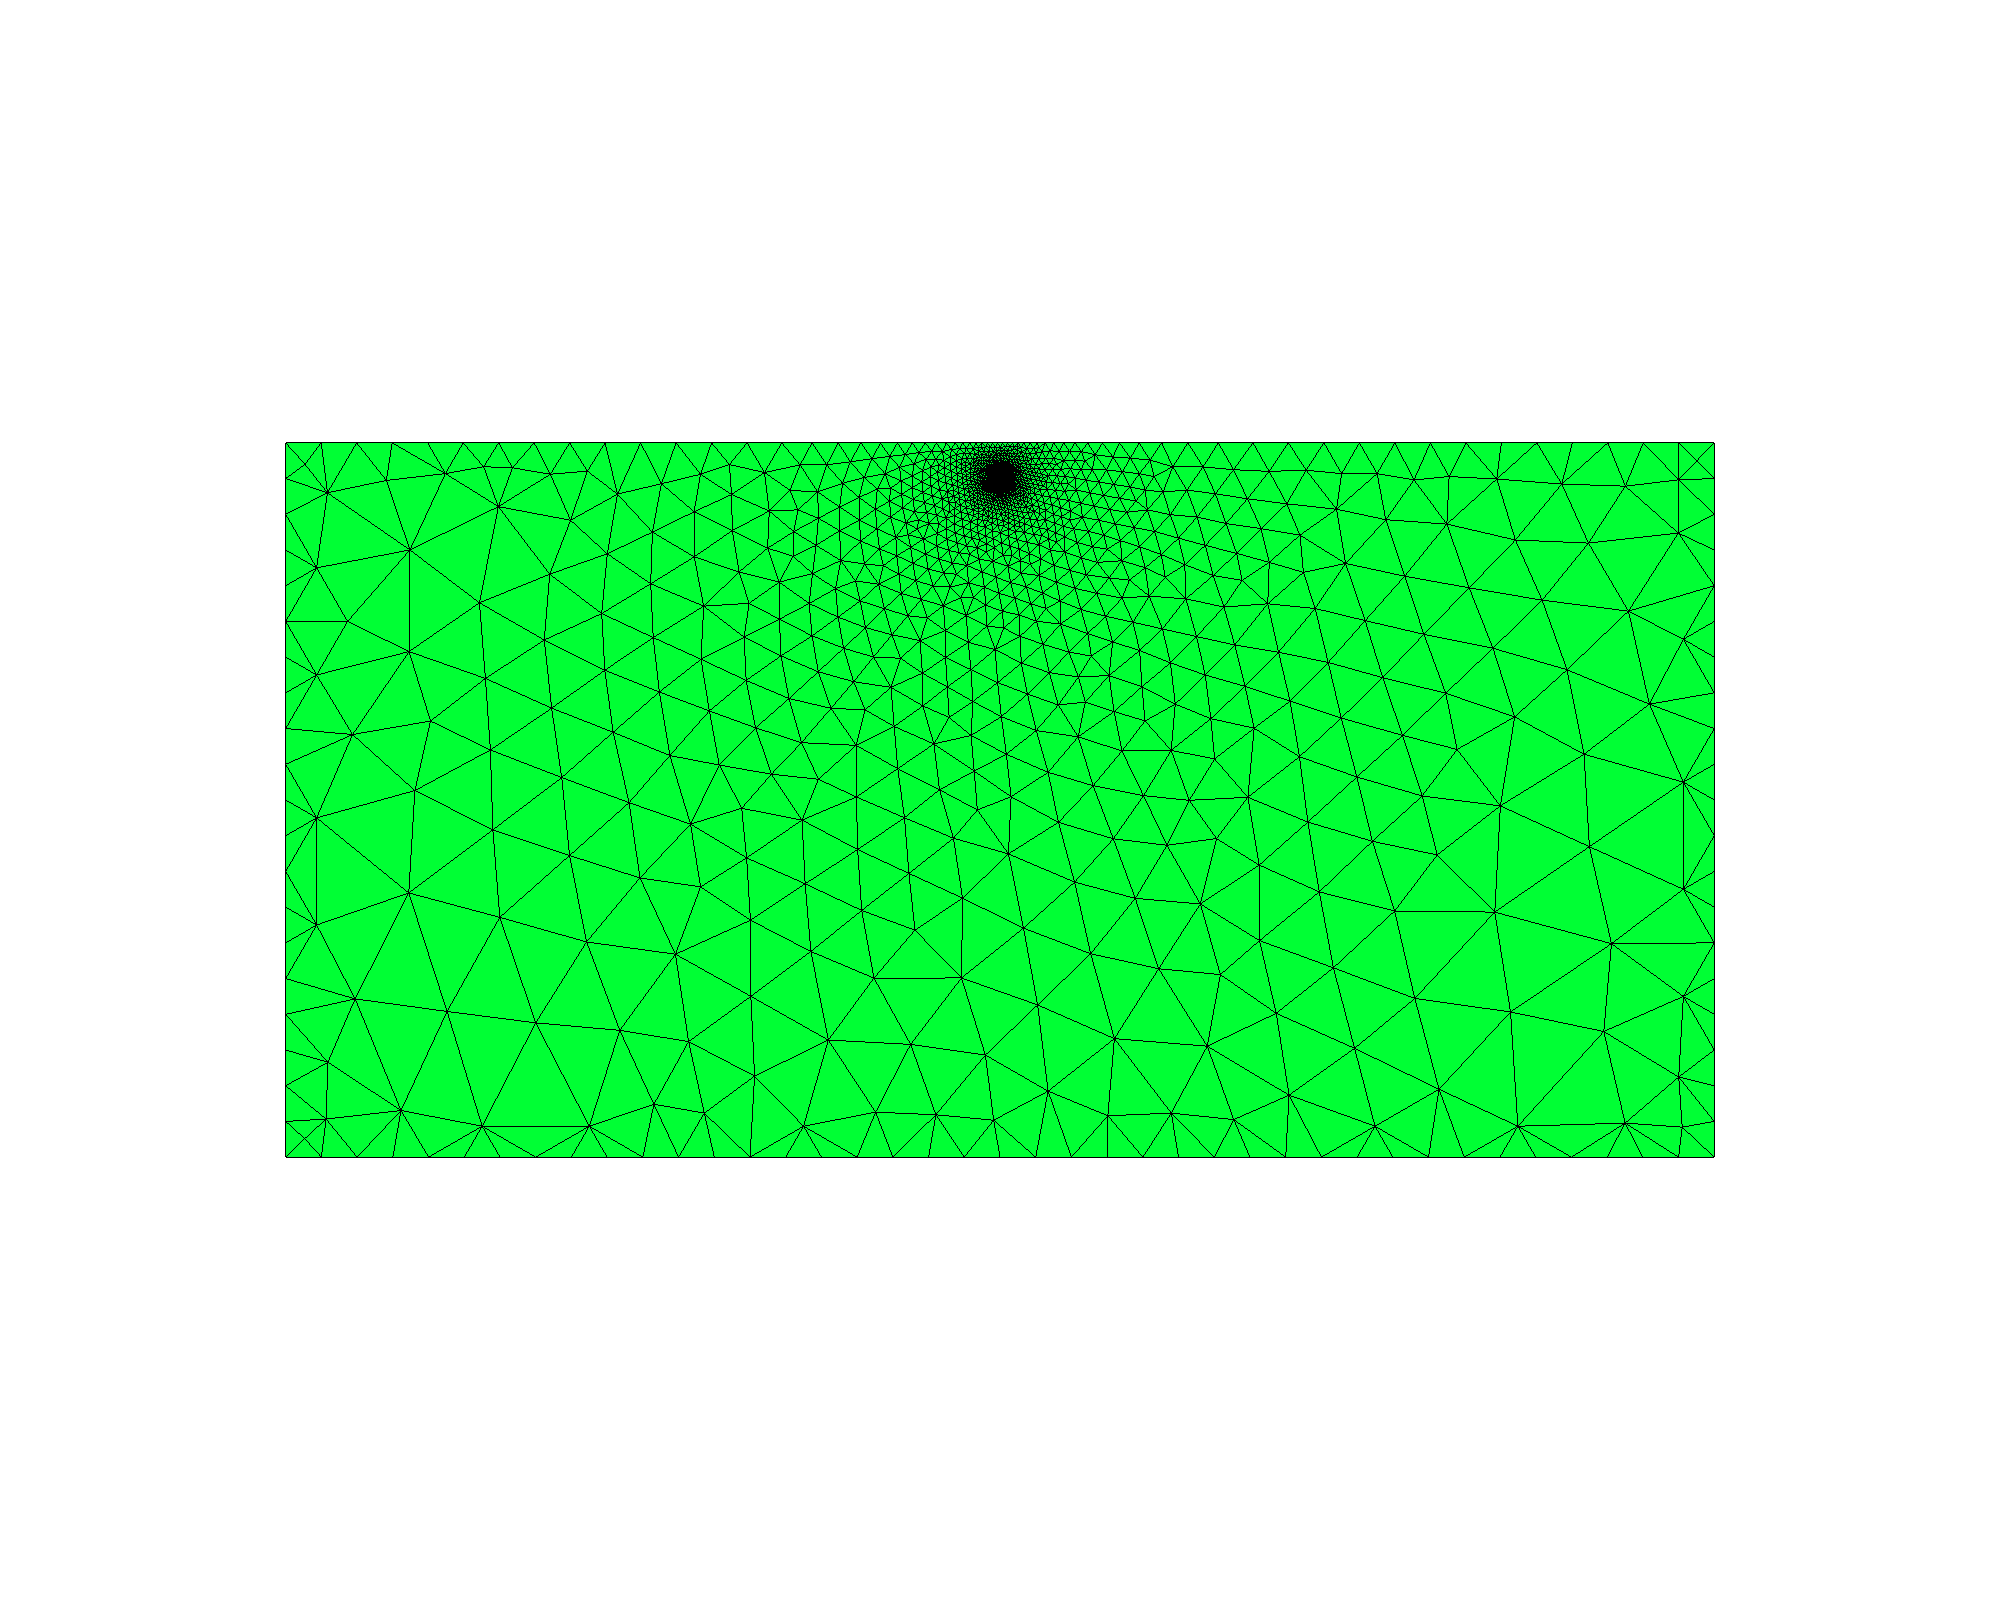
\includegraphics[width=\linewidth,trim=0 100 0 100,clip]{figures/mesh_domain.png}
\end{columns}
\end{frame}

\begin{frame}{Q4.3 Ambient, mesh and domain size}
\small $T_{\rm amb}$ = 15\,$^\circ$C (NKT rating) for air and deep soil.\\[4pt]
\begin{tabular}{@{}lrr@{}}\toprule
$\sigma(T)$ model & $T_{\max}$ [$^\circ$C] & iterations\\\midrule
MeshFactor 2 / 1 / 0.5 & \Tcnlcoarse\ / \Tcnl\ / \Tcnlfine & \Nitnlcoarse\ / \Nitnl\ / \Nitnlfine\\
Domain 10 / 20 / 40 m & \Tcnldomten\ / \Tcnl\ / \Tcnldomforty & \Nitnldomten\ / \Nitnl\ / \Nitnldomforty\\\bottomrule
\end{tabular}
\end{frame}

\begin{frame}{Q4.4 Temperature in the cable}
\begin{columns}[T]\column{0.45\textwidth}\centering\map{\linewidth}{t_cables_nl}
\column{0.55\textwidth}\small Hot spot \Tcnl\,$^\circ$C in the aluminium (isothermal to 0.01 K); the XLPE at the conductor screen is $\approx$\dTsemi\ K cooler (drop across the 0.4 mm semicon).
NKT and IEC limit: 90\,$^\circ$C continuous. At 350 A the FE is \emph{at} the limit: the rating is confirmed, with no margin.
\end{columns}
\end{frame}

\begin{frame}{Q4.5 Temperature around the cable and at the surface}
\begin{columns}[T]\column{0.4\textwidth}\centering\map{\linewidth}{t_soil_nl}
\column{0.6\textwidth}\plot{\linewidth}{3.8cm}{surface_profile}\\\small
Max.\ surface \Tsnl\,$^\circ$C ($h$=10). Isothermal surface: conductor \Tcnliso\,$^\circ$C (convection adds \dTcIso\ K).
\end{columns}
\end{frame}

\begin{frame}{Q4.6 Validation vs IEC 60287}
\small IEC ladder at 350 A: $\theta_c$ = \IecTheta\,$^\circ$C (ampacity \IecAmp\ A at 90\,$^\circ$C);
FE isothermal \Tcnliso, FE convective \Tcnl. Differences: surface condition, Kennelly + empirical trefoil
factor vs 2D conduction, FE screen losses (circulating + eddy), 0.5 mm gap, finite domain.
\end{frame}

\begin{frame}{Q4.7 Convergence of the nonlinear coupling}
\begin{columns}[T]\column{0.55\textwidth}\plot{\linewidth}{4.4cm}{nl_history}
\column{0.45\textwidth}\small Criterion: $\|T_k-T_{k-1}\|_2/\|T_k\|_2<10^{-6}$, all nodal $T$ (GetDP \texttt{GetNormIncrement}).
\Nitnl\ iterations; same with MeshFactor 2 and 0.5. Linear (fixed-point) convergence, factor $\approx$\ConvRate.
\end{columns}
\end{frame}

\begin{frame}{Q4.8 Linear vs $\sigma(T)$: maps and values}
\begin{columns}[T]
\column{0.14\textwidth}\centering\map{\linewidth}{t_cables_lin}\\{\tiny $T$ linear}\\[2pt]\map{\linewidth}{t_cables_nl}\\{\tiny $T$ $\sigma(T)$}
\column{0.14\textwidth}\centering\map{\linewidth}{m_j}\\{\tiny $|J|$ linear}\\[2pt]\map{\linewidth}{m_j_nl}\\{\tiny $|J|$ $\sigma(T)$}
\column{0.14\textwidth}\centering\map{\linewidth}{m_b}\\{\tiny $|B|$ linear}\\[2pt]\map{\linewidth}{m_b_nl}\\{\tiny $|B|$ $\sigma(T)$}
\column{0.58\textwidth}\scriptsize
\begin{tabular}{@{}lrrr@{}}\toprule
& linear & $\sigma(T)$ & change\\\midrule
$P$ cond.\ [kW/km] & \Pclin & \Pcnl & \dPcNL\%\\
$P$ screens [kW/km] & \Pslin & \Psnl & \dPsNL\%\\
$R_{AC}$ [$\Omega$/km] & \Raclin & \Racnl & \dRacNL\%\\
$L$ [mH/km] & \Llin & \Lnl & \dLNL\%\\
$T_{\max}$ / surface [$^\circ$C] & \Tclin\ / \Tslin & \Tcnl\ / \Tsnl & \dTcNL\ K\\\bottomrule
\end{tabular}\\[4pt]
Significant: losses, $R_{AC}$, $T$ (resistivity +\RhoHot\% at \Tcnl\,$^\circ$C). Screen loss drops
($\lambda_1\approx X^2/R_s$). $B$ and $L$ barely change (currents imposed, $\mu_r=1$); $J$ slightly more uniform.
\end{columns}
\end{frame}

\begin{frame}{Q4.9 Is the linear model conservative?}
\small \textbf{No.} It uses $\sigma$ at 20\,$^\circ$C: the $\sigma(T)$ losses are \dPtNL\% higher and the hot spot \dTcNL\ K hotter.
A rating based on the linear model would allow \AmpLin\ A instead of \Amptrefoil\ A: the cable would run above 90\,$^\circ$C.
\end{frame}

\begin{frame}{Section 5 Arrangement and bonding}
\begin{columns}[T]\column{0.55\textwidth}\plot{\linewidth}{4.6cm}{arrangement}
\column{0.45\textwidth}\centering\map{\linewidth}{t_cables_flat70}\\{\scriptsize flat, 70 mm free distance}
\end{columns}
\end{frame}

\begin{frame}{Reproducibility}
\small
\begin{itemize}
\item Gmsh 4.15.2, GetDP 4.0.0-git-259f4c38; git tag \texttt{final}
\item \textbf{File $>$ Open} \texttt{Electrodynamic-analysis/cable.pro} or \texttt{Magnetothermal-analysis/cable.pro}, \textbf{Run}
\item \texttt{run\_all.sh}: every case (one line each, with its question)
\item Numbers: \texttt{Reports/collect\_values.py} $\rightarrow$ \texttt{values.tex}; nothing typed by hand
\end{itemize}
\end{frame}
\end{document}
